\documentclass[a4paper]{article}

\usepackage[english]{babel}
\usepackage[utf8]{inputenc}
\usepackage{amsmath}
\usepackage{graphicx}
\usepackage[colorinlistoftodos]{todonotes}

\title{Assignment Lewis Model}

\author{Tim Schrama}

\date{\today}

\begin{document}
\maketitle

The transition from a labour surplus economy to a mature economy.

Preparation: derivation of the Lewis model.
Before we turn to the main questions of the assignment, we first build up the Lewis model. We will derive the most important equations for reference later on. Start by writing down the seven formulas that form blueprint of the Lewis design:

\begin{equation}
Y_S=A_S L_S
\end{equation}
\begin{equation}
w_S=A_S\\
\end{equation}
\begin{align}
Y_M=A_M K^\alpha L_M ^{1-\alpha}\\
w_M=[1-\alpha]\frac{Y_M}{L_M}\\
L=L_M+L_S\\
w_M=\phi w_S\\
\dot{K}= s_\pi [Y_M-w_M L_M ]-\delta K
\end{align}

We presume the meaning of all variables are known by the reader. In short, there are two sectors, a subsistence sector (subscript s) and a mature sector (subscript m). Only the mature sector works with capital, which is accumulated by saving a part of ‘profits’ (perhaps profits is somewhat a misnomer, total income of capitalists is meant). Over time, labour moves from the subsistence sector to the mature sector as a response to the wage gap determined by $\phi$.

Static Equilibria.

First consider the labour market. Start with equation [3] and rewrite as follows to find an expression for $L_M$ that only depends on K:

\begin{align}
w_M=(1-\alpha)\frac{Y_M }{L_M}\\
\rightarrow L_M=(1-\alpha)\frac{Y_M }{w_M}\nonumber \\
\rightarrow L_M=\frac{(1-\alpha) A_M K^\alpha (L_M)^{1-\alpha} }{w_M}	\nonumber \\
\rightarrow L_M=\frac{(1-\alpha) A_M K^\alpha (L_M)^{1-\alpha} }{\phi w_S} \nonumber \\
\rightarrow L_M=\frac{(1-\alpha) A_M K^\alpha (L_M)^{1-\alpha} }{\phi A_S} \nonumber \\
\rightarrow L_M=K[\frac{(1-\alpha) A_M }{\phi A_S}]^{\frac{1}{\alpha}} \nonumber
\end{align}
Then by equation [5]:

\begin{equation}
L_S=L-L_M		\rightarrow		L_S=L-K[\frac{(1-\alpha) A_M }{\phi A_S}]^{\frac{1}{\alpha}}
\end{equation}

Both [8] and [9] are only valid if $L_M<L$. This is equivalent to:
\begin{equation}
K[\frac{(1-\alpha) A_M}{\phi A_S}]^{\frac{1}{\alpha}}<L	\\
\rightarrow	K<L[\frac{\phi A_S}{(1-\alpha) A_M}]^{\frac{1}{\alpha}}\equiv K^{\#}
\end{equation}

Where $K^{\#}$ is the amount of capital at the point where the economy reaches maturity: no longer any labour is employed in the subsistence sector. Next, turn to output. Using the labour market equilibria, we can rewrite equation [1] and [3]:
\begin{equation}
Y_S=A_S L_S=A_S L-A_S K[\frac{(1-\alpha) A_M}{\phi A_S}]^{\frac{1}{\alpha}} \\
\end{equation}
\begin{equation}
Y_M=A_M K^\alpha [L_M]^{1-\alpha}=A_M K^\alpha [K[\frac{(1-\alpha) A_M}{\phi A_S}]^{\frac{1}{\alpha}}]^{1-\alpha} \nonumber\\
\end{equation}
\begin{equation}
=K A_M [\frac{(1-\alpha) A_M}{\phi A_S}]^{\frac{1-\alpha}{\alpha}}
\end{equation}

Since we work with a Cobb-Douglas production function in the mature sector, profits simply equal a fraction $\alpha$ of $Y_M$:

\begin{equation}
Y_M-w_M L_M= \alpha Y_M=\alpha K A_M [\frac{(1-\alpha) A_M}{\phi A_S}]^{\frac{1-\alpha}{\alpha}}
\end{equation}

Finally, total output Y is defined as the sum of output in both sectors:
\begin{equation}
Y=Y_S+Y_M 	=A_S L-K A_S [\frac{(1-\alpha) A_M}{\phi A_S}]^{\frac{1}{\alpha}}+K A_M [\frac{(1-\alpha) A_M}{\phi A_S}]^{\frac{1-\alpha}{\alpha}} \nonumber
\end{equation}
\begin{equation}
=A_S L-KA_S (\frac{(1-\alpha) A_M}{\phi A_S })^{\frac{1}{\alpha}}+K A_S\frac{\phi}{1-\alpha}[\frac{(1- \alpha) A_M}{\phi A_S}]^{\frac{1}{\alpha}} \nonumber
\end{equation}
\begin{equation}
=A_S L+K A_S (\frac{(\frac{\phi}{(1-\alpha)}- 1)(1-\alpha)A_M}{\phi A_S})^{1-{\alpha}}
\end{equation}

Dynamics.

Above we have found formulations for labour supply (per sector), output, profits and wages as a function of K and a bundle of exogenous variables. Since equation [7] specifies how K moves over time, we can analyse the dynamics the mentioned factors. First substitute profits as given by [13] into the capital accumulation equation and rewrite in terms of growth rates.
\begin{align}
\dot{K}= s_\pi [Y_M-w_M L_M ]-\delta K= \alpha s_\pi K A_M [\frac{(1-\alpha)A_M}{\phi A_S}]^{\frac{1-\alpha}{\alpha}}-\delta K \nonumber \\
\rightarrow	\hat{K}=\alpha s_\pi A_M [\frac{(1-\alpha)A_M}{\phi A_S}]^{\frac{1-\alpha}{\alpha}}-\delta
\end{align}

Note how the growth rate of capital is completely determined by exogenous variables (i.e. it is just a constant). Labour supply in the mature sector grows at the same rate as capital (as long as  $L_M<L$):
\begin{align}
\dot{L_M}=\dot{K}[((1-\alpha)A_M/\phi A_S)]^(1/\alpha) \nonumber \\
\rightarrow \hat{L_M}=\frac{\dot{K}\frac{(1-\alpha)A_M}{\phi A_S}^{\frac{1}{\alpha}}}{K[\frac{(1-\alpha)A_M}{\phi A_S}]^{\frac{1}{\alpha}}}=\hat{K}
\end{align}

Subsistence sector income should shrink over time, feeding the growing mature sector with labour:
\begin{align}
\dot{Y_S}=-\dot{K}A_S [\frac{(1-\alpha)A_M}{\phi A_S}]^{\frac{1}{\alpha}} \nonumber \\
\rightarrow \hat{Y_S}=-\dot{K}A_S \frac{[\frac{(1-\alpha)A_M}{\phi A_S}]^{\frac{1}{\alpha}}}{A_S L-A_S K(\frac{(1-\alpha)A_M}{\phi A_S})^{\frac{1}{\alpha}}} \nonumber \\
=-\hat{K}A_S \frac{[\frac{(1-\alpha)A_M}{\phi A_S}]{\frac{1}{\alpha}}}{\frac{A_S L}{K}-A_S [\frac{(1-\alpha)A_M}{\phi A_S}]^{\frac{1}{\alpha}}} \\
\dot{Y_M}=\dot{K}A_M [\frac{(1-\alpha)A_M}{\phi A_S}]^{\frac{1-\alpha}{\alpha}} \nonumber \\
\rightarrow	\hat{Y_M}=\frac{\dot{K}A_M [\frac{(1-\alpha)A_M}{\phi A_S}]^{\frac{1-\alpha}{\alpha}}}{KA_M [\frac{(1-\alpha)A_M}{\phi A_S}]^{\frac{1-\alpha}{\alpha}}} \nonumber \\
=\hat{K}
\end{align}

Because both inputs in the mature sector grow at rate $\hat{K}$, income in the mature sector does as well. Moreover, since profits are just a fraction of mature income, it shares the same growth rate $\hat{K}$. We conclude this section by deriving total income growth.
\begin{align}
\dot{Y}=\dot{K} A_S (\frac{\phi}{1-\alpha}-1)\frac{(1-\alpha) A_M}{\phi A_S}^{\frac{1}{\alpha}} \nonumber \\
\rightarrow \hat{Y} =\frac{\dot{K} A_S (\frac{\phi}{1-\alpha}-1)\frac{(1-\alpha)A_M}{\phi A_S}^{\frac{1}{\alpha}}}{Y} \nonumber \\
\rightarrow \hat{Y} =\dot{K} A_S \frac{(\frac{\phi}{1-\alpha}-1)(\frac{1-\alpha}{\phi} \frac{A_M}{A_S} )^{\frac{1}{\alpha}}}{A_S L+K A_S (\frac{\phi}{1-\alpha}-1)(\frac{1-\alpha}{\phi} \frac{A_M}{A_S} )^{\frac{1}{\alpha}}} \nonumber \\
\rightarrow \hat{Y} =\hat{K} A_S \frac{(\frac{\phi}{1-\alpha}-1)(\frac{(1-\alpha)}{\phi}  \frac{A_M}{A_S} )^{\frac{1}{\alpha}}}{\frac{A_S L}{K}+A_S (\frac{\phi}{1-\alpha}-1)(\frac{(1-\alpha)}{\phi}  \frac{A_M}{A_S})^{\frac{1}{\alpha}}} \nonumber \\
\rightarrow \hat{Y} =\hat{K} A_S \frac{(\frac{\phi}{1-\alpha}-1)(\frac{1-\alpha}{\phi}  \frac{A_M}{A_S}) ^{\frac{1}{\alpha}}+\frac{A_S L}{K}-\frac{A_S L}{K}}{\frac{A_S L}{K}+A_S (\frac{\phi}{1-\alpha}-1)(\frac{1-\alpha}{\phi}  \frac{A_M}{A_S})^{\frac{1}{\alpha}}} \nonumber \\
\rightarrow \hat{Y} =\hat{K} (1-\frac{A_S L}{A_S L+K A_S (\frac{\phi}{1-\alpha}-1)(\frac{1-\alpha}{\phi}  \frac{A_M}{A_S})^{\frac{1}{\alpha}}} \nonumber \\
= \hat{K} [1- A_S \frac{L}{Y}]
\end{align}
Over time $A_S$ $L/Y$ becomes smaller, leading to an increasing growth rate of income.


A. Savings rate assumptions
The Lewis model assumes that a fixed fraction of profits is reinvested; the Solow model assumes that a fixed fraction of total income is reinvested. Let’s compare the two assumptions: How does the Lewis model change if the Solow assumption about savings rates is used and vice versa? Show the dynamics of the models.

When connecting the Solow model and the Lewis model, the main issue is the different approach both models take with respect to the saving rate. In order to illustrate this, we use the following notation:

$s$	the savings rate as a fraction of total income (i.e. $Y_M$ + $Y_S$ in case of the Lewis model).
$s_Ym$	the savings rate as a fraction of income in the mature sector (only relevant for Lewis).
$s_\pi$	the savings rate as a fraction of profits.

Superscript L and S are used when referring to the Lewis model and the Solow model, respectively. If we reformulate the general assumptions of both paradigms in these terms, the Solow model usually specifies $s^S$, whereas the Lewis model normally works with ${s_\pi}^L$. Now suppose, perhaps naively, that we equalize these saving rates, such that $s^S={s_\pi}^L$. To make these saving rates more easily comparable, we first rewrite ${s_\pi}^L$ in terms of a saving rate as a percentage of total income $s^L$. Note that:

\begin{equation}
s_\pi^L [Y_M-w_M L_M ]= \alpha s_\pi^L Y_M= \alpha s_\pi^L  \frac{Y_M}{Y} Y=s^L Y	\rightarrow s^L=\alpha s_\pi^L  \frac{Y_M}{Y}
\end{equation}

At the maturity point of the economy, where $K=K^{\#}$, it holds that $Y_M=Y$ by definition. Therefore $s^L={\alpha s_\pi}^L$ at the transition point between Lewis and Solow. Yet for $K>K^{\#}$, note that $s^S>{\alpha s_\pi}^L$, which implies that the graph of the saving rate as a function of $K$ makes a sudden hike at $K^{\#}$. Visually:

\begin{figure}
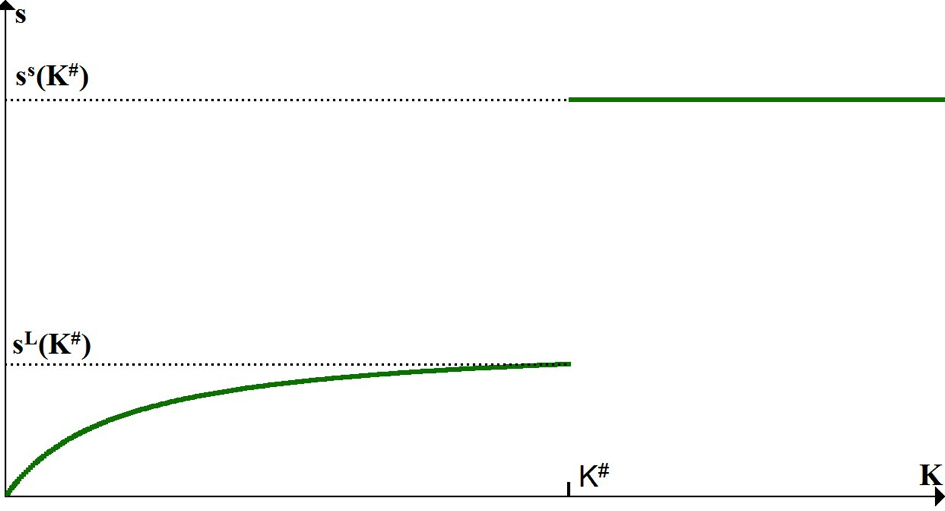
\includegraphics[width=\linewidth]{graph1.png}
\caption{\label{fig:Graph 1}saving rate as a function of $K$.}
\end{figure}

The saving rate is a smooth function over the Lewis range, i.e. $K<K^{\#}$, (it rises because the mature sector becomes an increasingly large part of the economy), but is discontinuous at the point where the Solow range is entered. There is no economic reason for this sudden hike and hence it is a problem we need to resolve if we want to link both models. Several possibilities are available.

I. Adjust the Solow model: save a fraction of “profits”.
In the Solow model, one could define savings on the basis of profits instead of total income: set $s_\pi^s=s_\pi^L$. We know that the total income of capitalists equals a fraction $\alpha$ of total income (as a result of the Cobb-Douglas production function). Hence, this adjustment comes down to setting $s^s= \alpha s_\pi^s$, a factor $\alpha$ lower than before. The gap in the savings function at $K^{\#}$ in graph 1 will disappears (see graph 2).

\begin{figure}
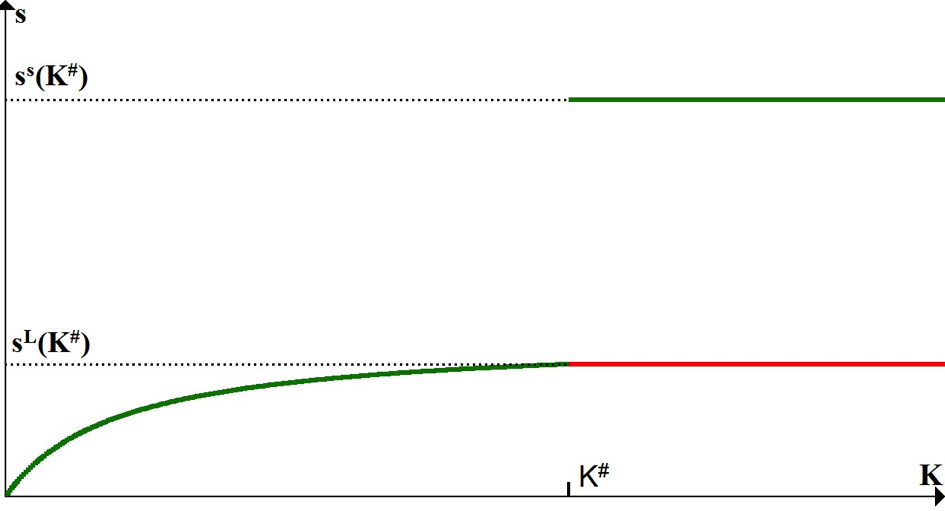
\includegraphics[width=\linewidth]{graph2.png}
\caption{\label{fig:Graph 2}In the Solow range, define savings on the basis of profits: $s$ shifts downward to the red line.}
\end{figure}

Obviously, the dynamics over the Lewis range remain unaltered, since no variable has changed in that dimension. With respect to the Solow range, the smaller saving fraction means that the rate of capital accumulation decreases…
\begin{equation}
\hat{K}= \alpha s^s k^{\alpha-1}-\delta<s^s k^{\alpha-1}-\delta
\end{equation}

\ldots as well as lowering the steady-state income level:

\begin{equation}
y^{\star} = \frac{\alpha s^s}{\delta}^{\frac{\alpha}{1-\alpha}}<\frac{s^s}{\delta}^{\frac{\alpha}{1-\alpha}}
\end{equation}

II. Adjust the Lewis model: save a fraction of total income in the maturity sector.
The reversed case is to use mature sector income $Y_M$ as the basis for savings in the Lewis model, i.e. $s_{Ym}= s^s$, mirroring the total income savings rate of the Solow model. Again, given the Cobb-Douglas production function, profits equal a fraction $\alpha$ of mature income. Thus, this modification is similar to selecting $s_\pi^L=\frac{s_{Ym}}{\alpha}$, inflating $s_\pi^L$ by a factor $1/\alpha$ compared to before. Graphically, the part of the savings curve before maturity is shifted upwards and the discontinuity has disappeared (see graph 3). 
From equation [15] it is clearly visible that the rate of capital growth increases by taking a broader basis for our savings. As a consequence, total income $Y_M+Y_S$ grows faster as well, see equation [19]. This change in dynamics over the Lewis range is displayed in graph 4. 

\begin{figure}
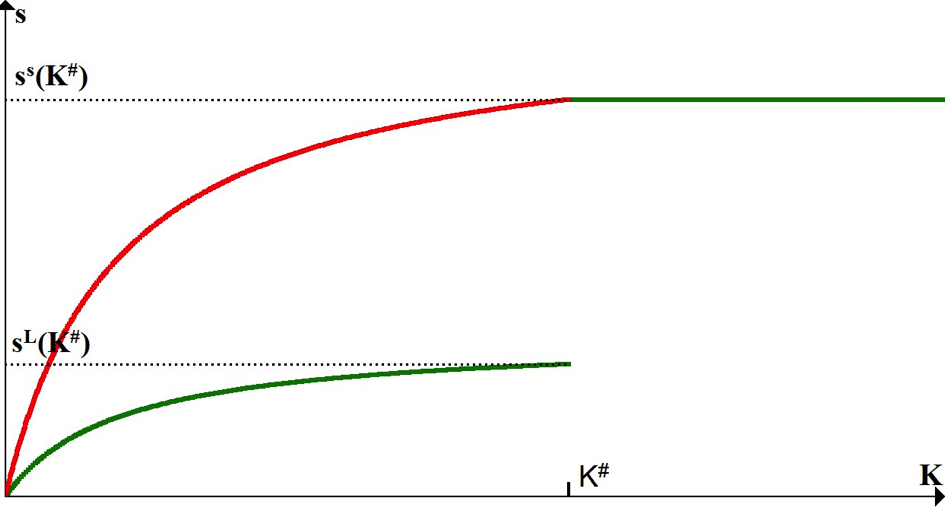
\includegraphics[width=\linewidth]{graph3.png}
\caption{\label{fig:Graph 3}In the Lewis range, define savings on the basis of mature income: $s$ shifts upward to the red line.}
\end{figure}

\begin{figure}
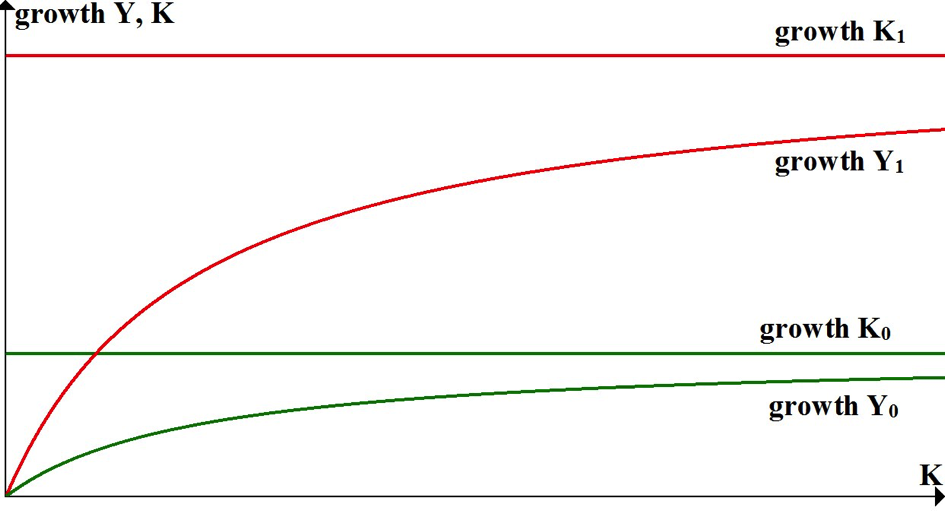
\includegraphics[width=\linewidth]{graph4.png}
\caption{\label{fig:Graph 4}Comparison of growth rates of $Y$ and $K$ (in the Lewis range): a savings rate based on profits (sub-script 0, green) versus a saving rate based on mature income (subscript 1, red).}
\end{figure}

III. Adjust the Lewis model: save a fraction of total income (in both sectors).
Instead of focussing solely on income in the mature sector, one could involve the subsistence sector as well: use $Y_M+Y_S$ as the basis for the saving rate in the Lewis model. This amounts to setting $s^L= s^s$.   As a percentage of total income, the savings rate in the Lewis range is now no longer increasing with $K$, instead it will be a constant function. Naturally this eliminates any discontinuity issues (see also graph 5). 
 
This adjustment has much larger consequences compared to the previous two cases: we have to reformulate the complete dynamics of the model, instead of simply changing one parameter. The capital accumulation equation now becomes:
\begin{align}
\dot{K}= s^L Y-\delta K= s^L A_S L+s^L K A_S (\frac{\phi}{1-\alpha}- 1)(\frac{(1-\alpha)A_M}{\phi A_S})^{\frac{1}{\alpha}}-\delta K \nonumber \\
\rightarrow \hat{K} =s^L A_S \frac{L}{K}+s^L A_S (\frac{\phi}{1-\alpha}- 1)(\frac{(1-\alpha)A_M}{\phi A_S})^{\frac{1}{\alpha}}-\delta 
\end{align}
Hence capital does no longer grow at a constant rate. Graph 6 shows what happens to the growth rate of capital and total income if we save a fixed fraction of total income.

\begin{figure}
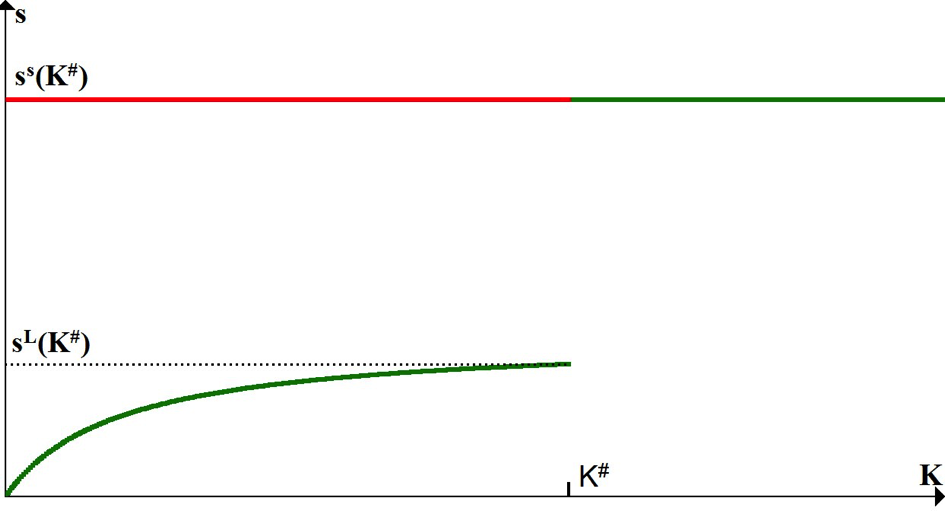
\includegraphics[width=\linewidth]{graph5.png}
\caption{\label{fig:Graph 5}In the Lewis range, define savings on the basis of total income: $s$ shifts upward to the red line.}
\end{figure}

\begin{figure}
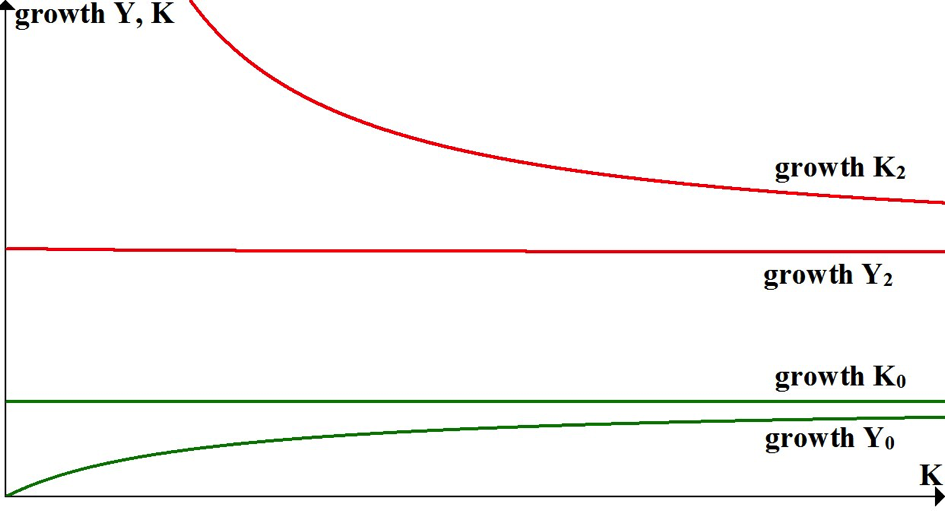
\includegraphics[width=\linewidth]{graph6.png}
\caption{\label{fig:Graph 6}Comparison of growth rates of $Y$ and $K$ (in the Lewis range): a savings rate based on profits (sub-script 0, green) versus a saving rate based on total income (subscript 2, red).}
\end{figure}

\end{document}